The XML benchmarking project XMARK~\cite{xmark/original} dataset is single record with large and complex tree structure. It is one of the most popular and most commonly used XML Benchmark~\cite{xmark/mlynkova2008xml}. It uses a small executable tool called  \textit{xmlgen} that enables to create a synthetic XML Dataset according to fixed DTD of an Internet auction database. The xmlgen produces the dataset that is platform independent and accurately scalable ranging from a minimal document to any arbitrary size limited by the capacity of the system. 
\subsubsection{Dataset}
\label{xmark-dataset}
	XMARK dataset is single record with huge and complicated tree structure ~\cite{xmark/VIST}. 
	%\tikzset{
	basic/.style  = {draw, text width=2cm, drop shadow, font=\sffamily, rectangle},
	root/.style   = {basic, rounded corners=2pt, thin, align=center,
		fill=green!30},
	level 2/.style = {basic, rounded corners=6pt, thin,align=center, fill=green!60,
		text width=8em},
	level 3/.style = {basic, thin, align=left, fill=pink!60, text width=6.5em}
}
\begin{tikzpicture}[
level 1/.style={sibling distance=40mm},
edge from parent/.style={->,draw},
>=latex]

% root of the the initial tree, level 1
\node[root] {Drawing diagrams}
% The first level, as children of the initial tree
child {node[level 2] (c1) {Defining node and arrow styles}}
child {node[level 2] (c2) {Positioning the nodes}}
child {node[level 2] (c3) {Drawing arrows between nodes}};

% The second level, relatively positioned nodes
\begin{scope}[every node/.style={level 3}]
\node [below of = c1, xshift=15pt] (c11) {Setting shape};
\node [below of = c11] (c12) {Choosing color};
\node [below of = c12] (c13) {Adding shading};

\node [below of = c2, xshift=15pt] (c21) {Using a Matrix};
\node [below of = c21] (c22) {Relatively};
\node [below of = c22] (c23) {Absolutely};
\node [below of = c23] (c24) {Using overlays};

\node [below of = c3, xshift=15pt] (c31) {Default arrows};
\node [below of = c31] (c32) {Arrow library};
\node [below of = c32] (c33) {Resizing tips};
\node [below of = c33] (c34) {Shortening};
\node [below of = c34] (c35) {Bending};
\end{scope}

% lines from each level 1 node to every one of its "children"
\foreach \value in {1,2,3}
\draw[->] (c1.195) |- (c1\value.west);

\foreach \value in {1,...,4}
\draw[->] (c2.195) |- (c2\value.west);

\foreach \value in {1,...,5}
\draw[->] (c3.195) |- (c3\value.west);
\end{tikzpicture}
	


\newpage
\begin{figure}
	\centering
	\subfigure[Reference in \textit{XMark} dataset tree Fig~\cite{xmark/original}]{
		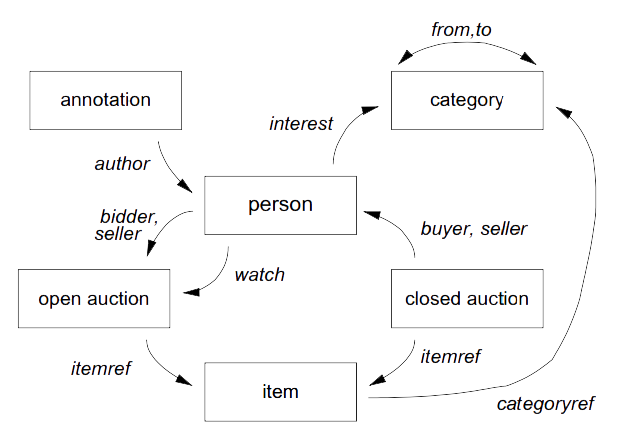
\includegraphics[width=0.40\textwidth]{img/xmark-references.png}{
			\label{xmark-reference}
		}
	}
	\centering
	\subfigure[Reference in \textit{XMark} dataset tree Fig~\cite{xmark/original}]{
		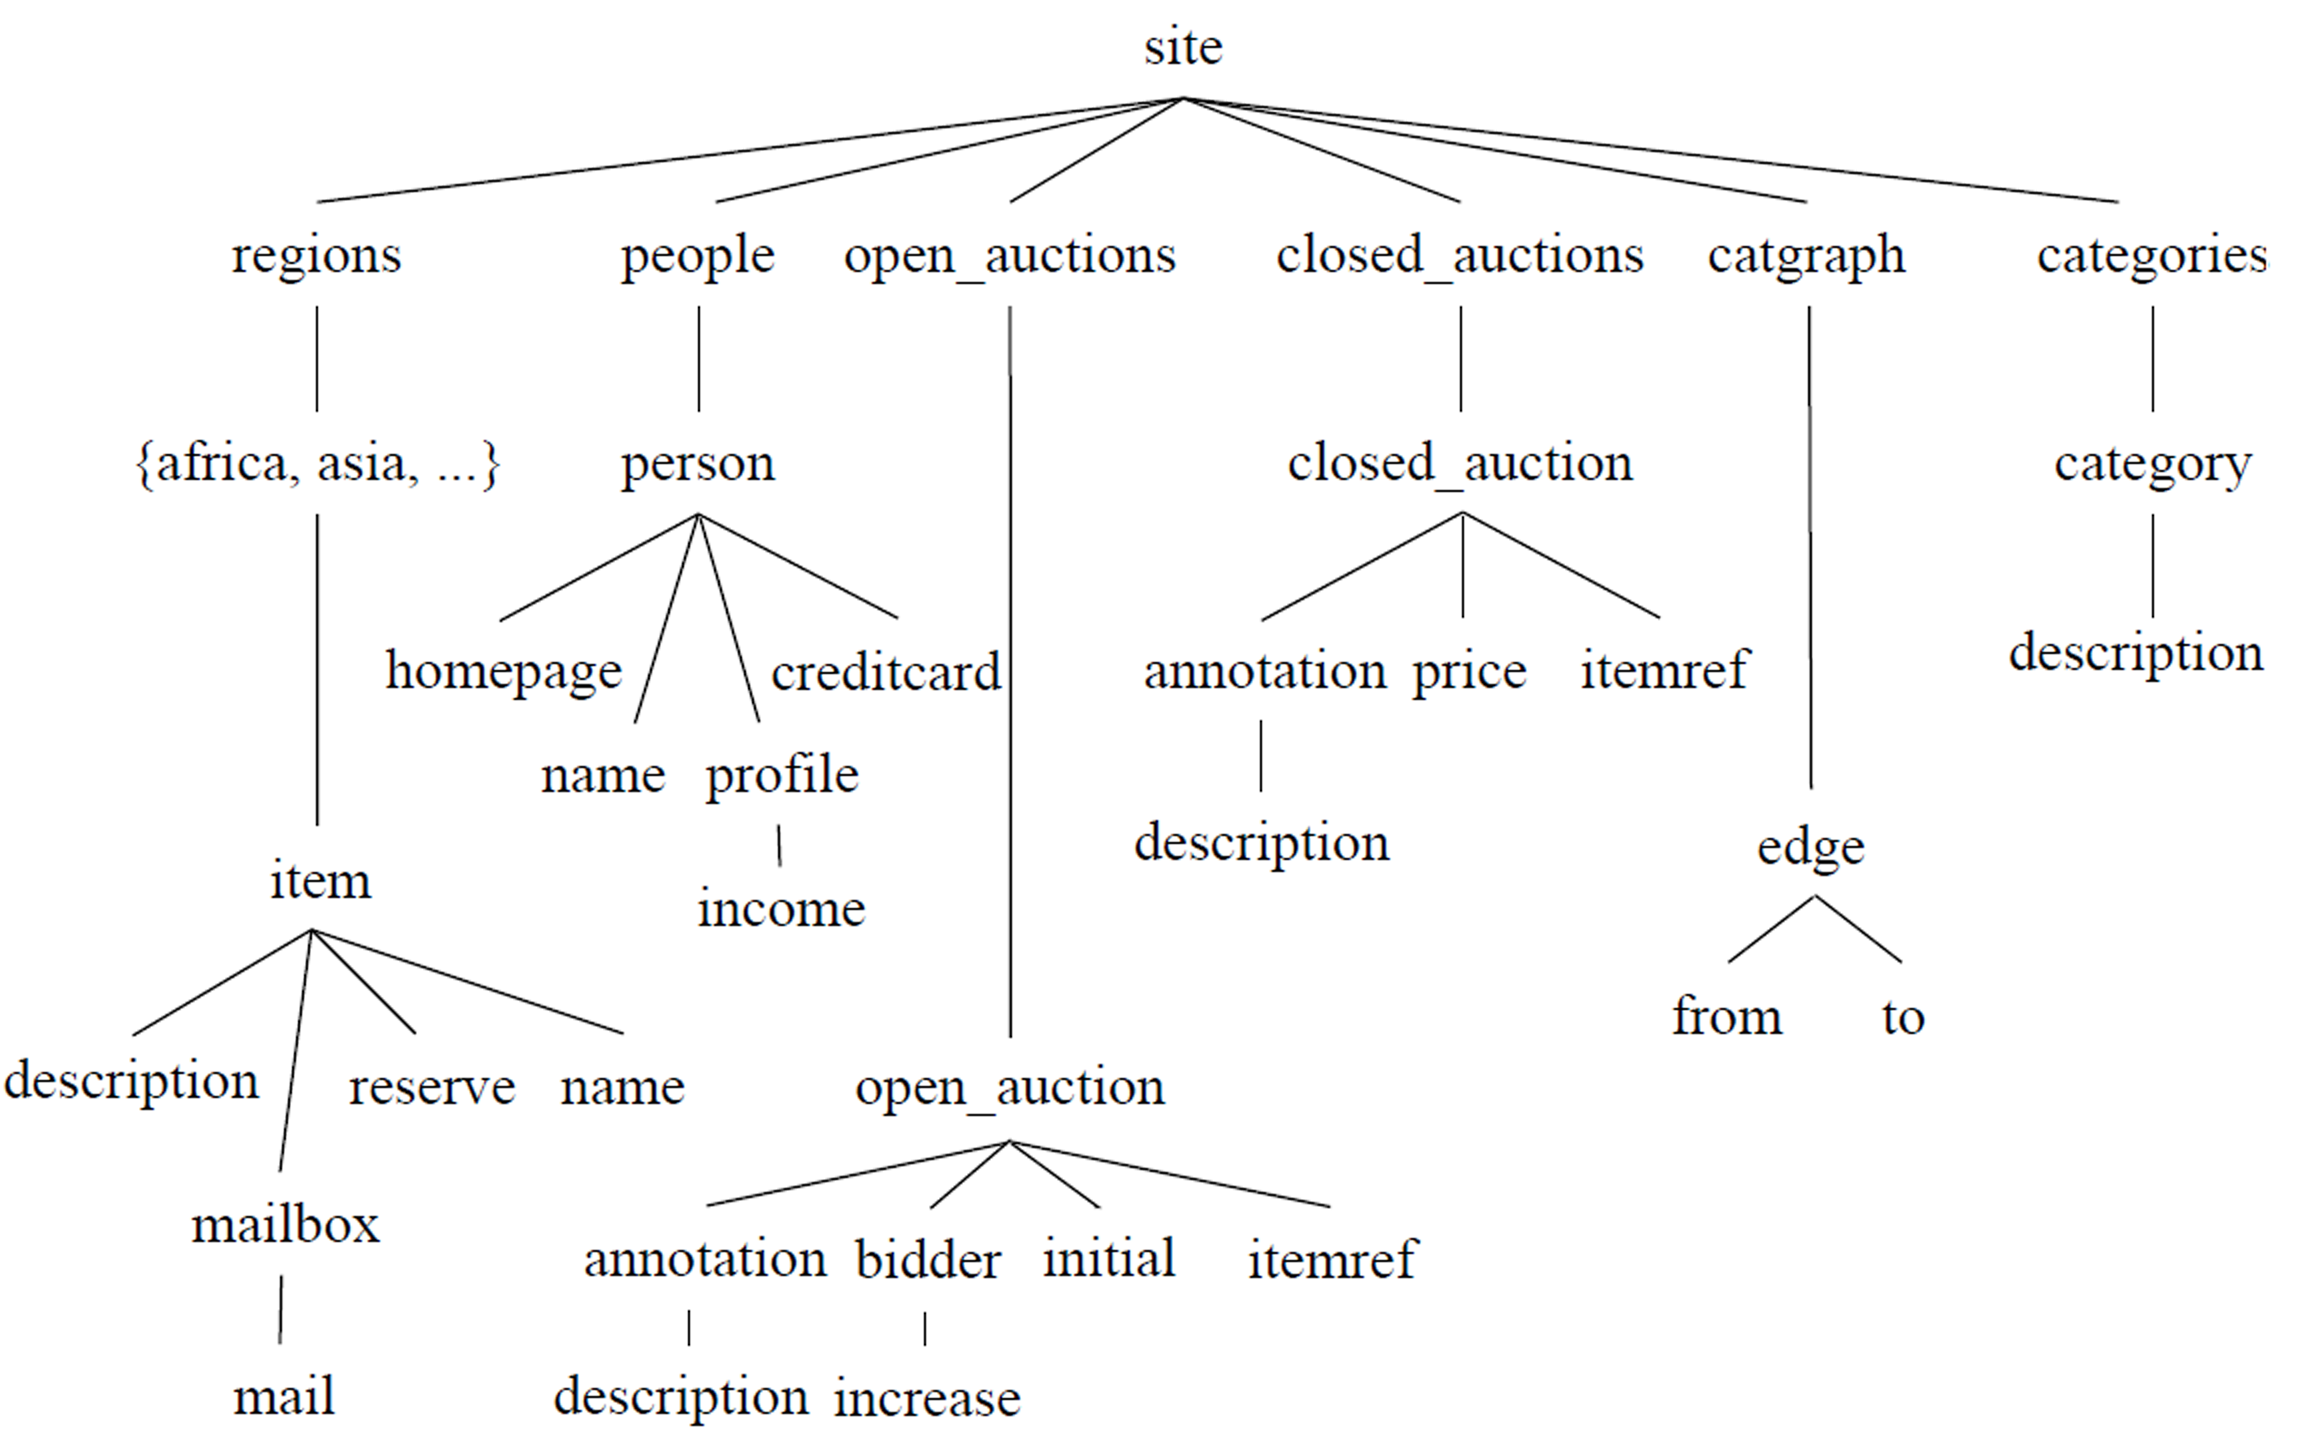
\includegraphics[width=0.40\textwidth]{img/xmark-tree.png}{
			\label{fig:xmark-tree}
		}
	}
	\caption{XMark data tree and reference}
	\label{fig:xmark-tree-reference}
\end{figure}
\begin{figure}
	\centering
	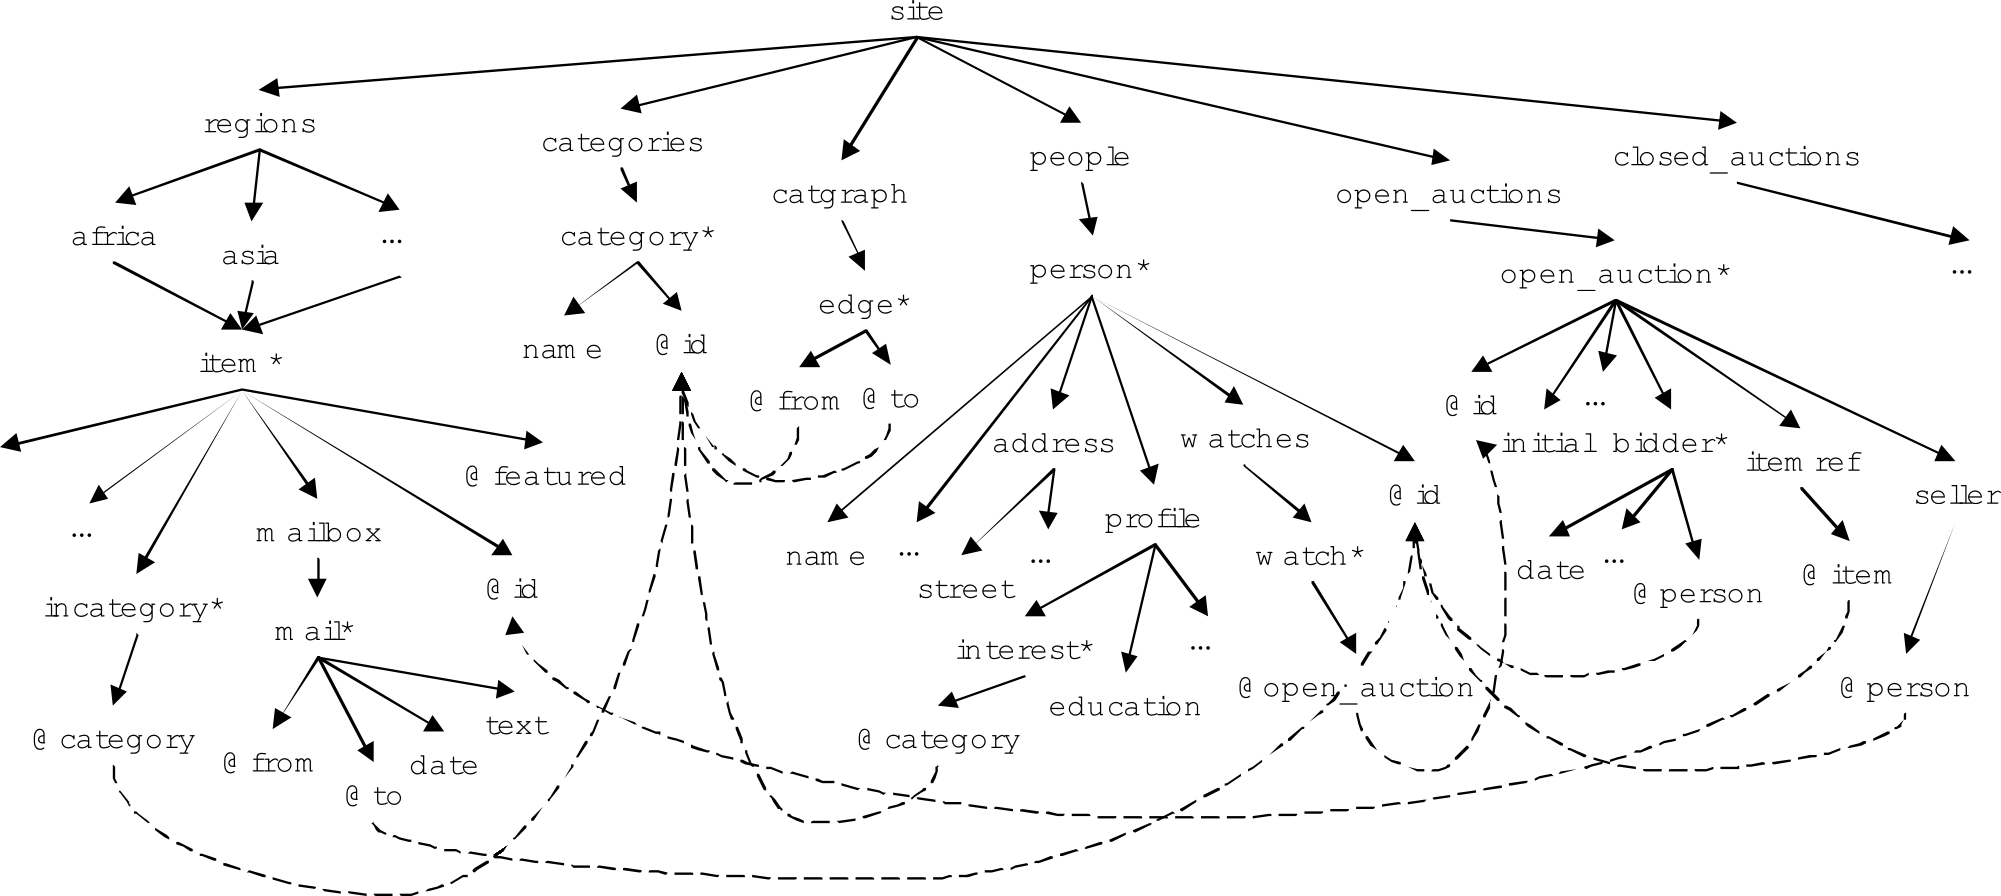
\includegraphics[width=0.40\textwidth]{img/xmark-schema.png}
	\caption{XMark schema with reference}\cite{xmark/schema-sumerize}
	\label{fig:xmark-schema}
\end{figure}

\todo{figure need to create}

\subsubsection{Queries}
\label{xmark-queries}
